\scanpage{15}
\mspage{6}

diagonales de l'hexagone, ou encore aux trois pts d'ordre 2 distincts de $e$.

Ici encore on peut ``doubler'' la décomposition cellulaire, et en \unsure{tirer} une autre avec 4 sommets, \deleted{\unsure{8|6}} \inserted{\unsure{12}} arêtes, et 8 faces (triangulaires), qui permet de mieux comprendre le passage au quotient par $\pm1$, avec quatre sommets (dont un sommet privilégié, correspondant à $e$),

\figure{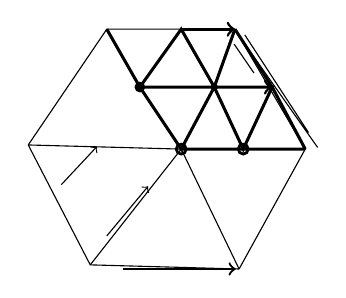
\begin{tikzpicture}[scale=1.05]
\coordinate (L) at (-1.85,0);
\coordinate (UL) at (-.9,1.4);
\coordinate (UR) at (.65,1.4);
\coordinate (R) at (1.5,-.05);
\coordinate (LR) at (.7,-1.5);
\coordinate (LL) at (-1.1,-1.45);
\coordinate (O) at (0,-.05);
\coordinate (T) at (0,1.4);
\coordinate (P) at (-.5,.7);
\coordinate (Q) at (.4,.7);
\coordinate (V) at (1.1,.7);
\coordinate (W) at (.75,-.05);
\draw (L)--(UL)--(UR)--(R)--(LR);
\draw (LR)--(LL)--(L);
\draw (L)--(O)--(LL) (O)--(LR);
\draw[line width=1.1pt] (UL)--(P)--(O)--(Q)--(UR);
\draw[line width=1.1pt] (P)--(T)--(Q)--(W)--(V)--(Q)--(P);
\draw[line width=1.1pt] (O)--(W)--(R) (UR)--(V)--(R);
\draw[->,line width=1pt] (T)--(UR);
\draw[->,line width=1pt] (Q)--(V);
\draw[->] (-1.45,-.48)--(-1.02,-.02);
\draw[->] (-.9,-1.1)--(-.4,-.5);
\draw[->,line width=.8pt] (-.7,-1.5)--(.66,-1.5);
\draw[thin] (.70,1.32)--(1.65,-.03) (.77,1.33)--(1.54,.15) (.64,1.22)--(.88,.87);
\fill (P) circle (.065);
\fill (Q) circle (.045);
\draw[line width=1pt] (O) circle (.06) (W) circle (.06);
\end{tikzpicture}}

six arêtes les reliant $2\unsure{:|à}2$ : c'est la structure tétraédrique \inserted{(orientée)}, avec un sommet fixé, groupe \unsure{d'automorphismes|d'automorphisme} $\mathbb Z/3\mathbb Z$ (\deleted{\unsure{pourtant}} $\simeq\mathbb Z/6\mathbb Z\,/\pm1$, OK !).

\margin{14}
